\section{Experiments}

\subsection{Dataset}
\label{subsec:dataset}
Due to its commercial value, real-life SC systems such as Uber and TaskRabbit do not make their datasets available to public. For this reason, we generate a realistic streaming workload based on the ideas in \cite{Tang07}. To generate a workload suitable for SC systems we have to model three different sets of parameters:\\
\textbf{Temporal Parameters:} In \cite{Basu15}, it's shown that in crowdsourcing environments, workers and tasks arrive following a Poisson process\textcolor{red}{\textbf{ref to Poisson process}}. For our experiments, unless stated otherwise, tasks and workers arrive based on a Poisson process with an arrival rate of $\mu_t = 250/hour$ and $\mu_w = 40/hour$ respectively.\\
\textbf{Spatial Parameters:} Former studies on the SC framework \cite{Kazemi12, Kazemi13, Deng13} have used datasets such as Gowalla\footnote{\url{snap.stanford.edu/data/loc-gowalla.html}} and Yelp\footnote{\url{www.yelp.com/data_challenge/}}  to model the location of the tasks in an SC environment. As shown in \textcolor{red}{\textbf{ref Hien's paper}}, the location of the tasks are not uniformly distributed. Rather, the spatial distribution of tasks are skewed, meaning that the density of the tasks in certain areas is higher. To model the same effect in our workload, 80\% of the tasks are located within 6 Gaussian clusters. The mean and standard deviation of the clusters are selected randomly. The locations of the remaining 20\% of the tasks are uniformly selected. Also, we assume the workers are uniformly distributed in the entire area under study.\\
\textbf{Static Parameters:} In addition to the spatiotemporal parameters discussed here, there exists a few other parameters that are generated as follows:\\
\emph{Workload Size:} Unless stated otherwise, each experiment runs on 10K tasks. The task arrival rate and the number of tasks determine the duration of the simulation. Based on the duration of the simulation and the worker arrival rate, the total number of workers may vary.\\
\emph{Grid Size:} We assume the simulation is run in a $36 \times 36\ mile^2$ area. For the algorithms requiring a grid, the entire area is divided into a $10 \times 10$ grid with equally sized cells.\\
\emph{$w_{max}$:} The maximum number of tasks a worker can perform is a uniformly random number from the closed interval $\left[8,12 \right]$.

\subsection{Online Vs. Offline}
In the first set of experiments, we compare how the results of different online algorithms compare with the optimal solution computed using the offline clairvoyant algorithm explained in \cref{sec:exactalgo}. Because of the high complexity of the offline algorithm, we were not able to run tests with large workloads. The experiments in this section were conducted using workload with 100 tasks.

\begin{figure}[h]
	\centering
	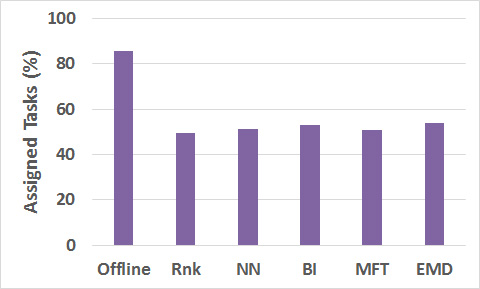
\includegraphics[width = 0.6\columnwidth]{figures/off_vs_on.jpg}
	\vspace{-0.1in}
	\caption{Online Vs. Offline}\label{fig:off_vs_on}
\end{figure}

The experimental results in \cref{fig:off_vs_on} show that the online algorithms perform within \%55-65 of the optimal solution. These experimental results are consistent with studies that indicate in the online assignment problem with random inputs, greedy algorithms achieve a competitive ratio of $1 - \frac{1}{e}$ \textcolor{red}{\textbf{provide ref}}.

\subsection{Performance}
In this section we evaluate the performance of different online non-clairvoyant algorithms explained in \cref{sec:onlinealgo}. First we compare them using the default parameters of \cref{subsec:dataset}. After that we show how the spatial and temporal aspects of the problem can affect the performance of the real-time assignments.

\begin{figure}[h]
	\centering
	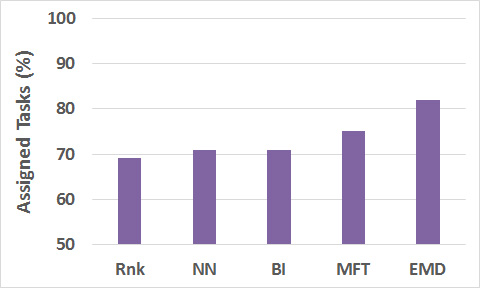
\includegraphics[width = 0.6\columnwidth]{figures/accuracy.jpg}
	\vspace{-0.1in}
	\caption{Accuracy of online algorithms}\label{fig:accuracy}
\end{figure}

\cref{fig:accuracy} compares the performance of different online algorithms. As we can see, our proposed EMD algorithm can assign \%10-15 more tasks compared to other approaches. The main reason as explained in \cref{sec:onlinealgo} is that, the EMD algorithm utilizes a very limited knowledge of the location of future tasks. It tends to send workers to areas where there's a higher chance of a task showing up in the future. This will increase the likelihood of a worker being close to those potential tasks once they arrive.

\begin{figure}[h]
	\centering
	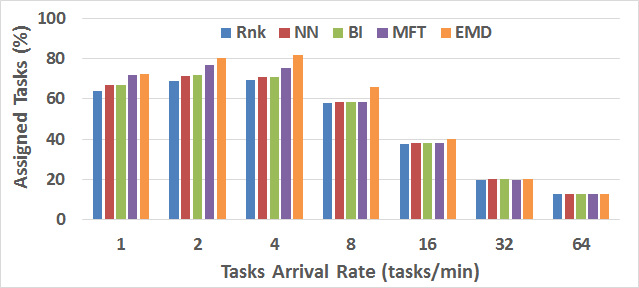
\includegraphics[width = 0.9\columnwidth]{figures/accuracy_trate.jpg}
	\vspace{-0.1in}
	\caption{Effect of task arrival rate}\label{fig:trate}
\end{figure}

In \cref{fig:trate} and \cref{fig:wrate} we show the effect of increasing the arrival rate of tasks and workers respectively. These results show when there are too many tasks (high task arrival rates) we eventually get to a point where all workers are executing at their full capacity and cannot accept more tasks. On the other end, when we have too many workers (high worker arrival rate) every task can be assigned to at least one worker. However, when we are not in either of the two extremes, the EMD algorithm outperforms other approaches by up to \%15.

\begin{figure}[h]
	\centering
	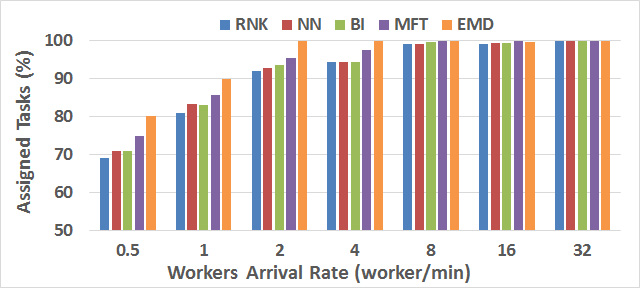
\includegraphics[width = 0.9\columnwidth]{figures/accuracy_wrate.jpg}
	\vspace{-0.1in}
	\caption{Effect of worker arrival rate}\label{fig:wrate}
\end{figure}

\cref{fig:trate,fig:wrate} showed the effects of temporal parameters in the performance of online SC algorithms. In \cref{fig:skewness} we show how the spatial skewness of tasks can affect the performance of online approaches. As explained in \cref{subsec:dataset}, our workload generator places \%80 of the tasks within 6 Gaussian clusters. In these set of experiments, we change the percentage of tasks located within the 6 random Gaussian clusters. Overall, as we increase the spatial skewness of tasks, all approaches perform better. The reason is that workers that end up being in the clusters, can complete a large number of tasks. The EMD algorithm tends to take more advantage since it's designed to send the workers from areas with fewer tasks to these high density clusters.

\begin{figure}[h]
	\centering
	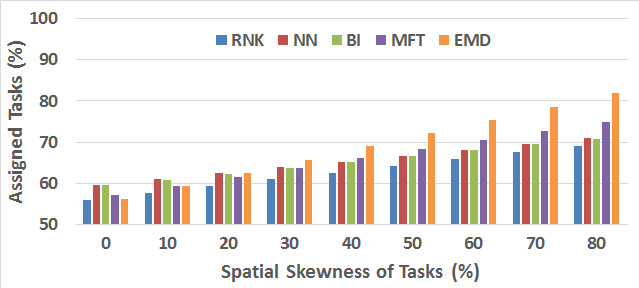
\includegraphics[width = 0.9\columnwidth]{figures/accuracy_skewness.jpg}
	\vspace{-0.1in}
	\caption{Effect of spatial skewness of tasks}\label{fig:skewness}
\end{figure}

\subsection{Scalability}
The last set of experiments tend to measure the scalability of the proposed framework in \cref{sec:onlinealgo} on various aspects. First we show that the size of the workload is irrelevant in the performance of the online algorithms. Following that we show the affect of task/worker arrival rate in our framework.

The first set of experiments in this part focus on the size of the workload; i.e., the total number of tasks. Increasing the workload size, will only increase the duration of the simulation.

\begin{table}[h]
\begin{center}
\begin{tabular}{| l || c | c | c | c | c |} \hline
Workload Size	&	Rnk		&	NN		&	BI		&	MFT		&	EMD		\\ \hline
1K				&	70.44	&	74.64	&	74.6	&	74.56	&	76.52	\\ \hline
10K				&	70.62	&	74.12	&	74.02	&	76.32	&	78.78	\\ \hline
100K			& 	69.95	&	73.13	&	73.13	&	76.55	&	78.52	\\ \hline
1M				&	70.22	&	74.41	&	74.58	&	77.18	&	79.12	\\ \hline
\end{tabular}
\vspace{-0.1in}
\caption{\small{\% of assigned tasks for different workload sizes}}
\label{tab:size_perc}
\end{center}
\end{table}
\vspace{-0.3in}
\begin{table}[h]
\begin{center}
\begin{tabular}{| l || c | c | c | c | c |} \hline
Workload Size	&	Rnk		&	NN		&	BI		&	MFT		&	EMD		\\ \hline
1K				&	0.38	&	0.34	&	0.42	&	0.49	&	12.28	\\ \hline
10K				&	0.40	&	0.34	&	0.43	&	0.41	&	10.72	\\ \hline
100K			& 	0.46	&	0.34	&	0.43	&	0.53	&	12.47	\\ \hline
1M				&	0.45	&	0.35	&	0.44	&	0.51	&	12.92	\\ \hline
\end{tabular}
\vspace{-0.1in}
\caption{\small{average time (ms) required to assign a single task}}
\label{tab:size_time}
\end{center}
\end{table}
\vspace{-0.3in}
\begin{table}[h]
\begin{center}
\begin{tabular}{| l || c | c | c | c | c |} \hline
Workload Size	&	Rnk		&	NN		&	BI		&	MFT		&	EMD		\\ \hline
1K				&	51.58	&	35.75	&	35.50	&	50.09	&	53.94	\\ \hline
10K				&	53.80	&	35.13	&	35.00	&	51.80	&	54.98	\\ \hline
100K			& 	53.03	&	35.17	&	34.94	&	51.10	&	54.37	\\ \hline
1M				&	54.39	&	35.58	&	35.38	&	51.27	&	55.79	\\ \hline
\end{tabular}
\vspace{-0.1in}
\caption{\small{average traveled distance (mile) per completed task}}
\label{tab:size_dist}
\end{center}
\end{table}

\cref{tab:size_perc,tab:size_time,tab:size_dist} show the percentage of assigned tasks, average run-time to assign a task and average traveled distance per completed task do not change significantly even if the workload size is increased by orders of magnitude.

In practice, our proposed framework for the online algorithms acts similar to a \emph{complex event processing (CEP)} engine \cite{Luckham01}. We can measure the scalability of such systems by their throughput; the number of tasks processed per second. The results in \cref{tab:size_time} are averaged over the tasks that we assigned to a worker. For tasks that could not be assigned to workers, the run-time is less, specially in the case of EMD the difference is significant ($\sim 0.4 ms$). To measure the throughput of such systems, the best way is to measure the queuing delay of tasks once they arrive \cite{Wu06}. In \cref{fig:qdelay} we see the average queuing delay of tasks after running the framework for 1 hour. As we can see, with the EMD we start observing queuing delays once we get to \textasciitilde 200 tasks/sec. While this is still an acceptable number for most current applications, it's less scalable than other approaches.

\begin{figure}[h]
	\centering
	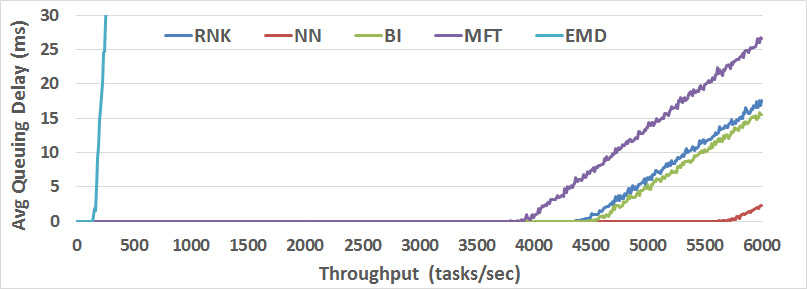
\includegraphics[width = 0.9\columnwidth]{figures/queue_delay.jpg}
	\vspace{-0.1in}
	\caption{Average queuing delay}\label{fig:qdelay}
\end{figure}

We end this section with a discussion on the effect of worker arrival rate on the scalability of the online approaches. In our proposed framework each worker can compute its own bid independently. Therefore, this process is done in parallel and increasing the number of workers will not affect the duration of the bid computation phase. Once all the workers submit their bids to the SC server, the server has to select the winner by either finding the minimum or maximum bid depending on which approach it's using. This will only add \emph{log|W|} to the processing time which is negligible. Hence, increasing the arrival rate of the workers will not have an affect on the scalability of our proposed framework regardless of which approach is being used.